% -*- TeX:de -*-
\NeedsTeXFormat{LaTeX2e}
\documentclass[12pt,a4paper]{article}
\usepackage[german]{babel} % german text
\usepackage[DIV12]{typearea} % size of printable area
\usepackage[T1]{fontenc} % font encoding
%\usepackage[latin1]{inputenc} % most likely on Windows
\usepackage[utf8]{inputenc} % probably on Linux
\usepackage{multicol}

% PLOTTING
\usepackage{pgfplots} 
\usepackage{pgfplotstable}
\usepackage{url}
\usepackage{graphicx} % to include images
\usepackage{tikz}
\usepackage{subfigure} % for creating subfigures
\usepackage{amsmath} % a bunch of symbols
\usepackage{amssymb} % even more symbols
\usepackage{booktabs} % pretty tables
\usepackage{makecell} % multi row table heading

% a floating environment for circuits
\usepackage{float}
\usepackage{caption}

%\newfloat{circuit}{tbph}{circuits}
%\floatname{circuit}{Schaltplan}

% a floating environment for diagrams
%\newfloat{diagram}{tbph}{diagrams}
%\floatname{diagram}{Diagramm}
\pgfplotsset{compat=1.8}
\selectlanguage{german} % use german

\begin{document}

%%%%%%% DECKBLATT %%%%%%%
\thispagestyle{empty}
			\begin{center}
			\Large{Fakultät für Physik}\\
			\end{center}
\begin{verbatim}


\end{verbatim}
							%Eintrag des Wintersemesters
			\begin{center}
			\textbf{\LARGE SS 14}
			\end{center}
\begin{verbatim}


\end{verbatim}
			\begin{center}
			\textbf{\LARGE{Physikalisches Praktikum\\ für das Bachelorstudium}}
			\end{center}
\begin{verbatim}




\end{verbatim}

			\begin{center}
			\textbf{\LARGE{PROTOKOLL}}
			\end{center}
			
\begin{verbatim}

\end{verbatim}

			\begin{flushleft}
			\textbf{\Large{Experiment (Nr., Titel): PS12 - Magnetismus}\\
							%Experiment Nr. und Titel statt den Punkten eintragen
			\LARGE{PS12}}	
			\end{flushleft}

\begin{verbatim}

\end{verbatim}	
							%Eintragen des Abgabedatums, oder des Erstelldatums des Protokolls
			\begin{flushleft}
			\textbf{\Large{Datum:}} \Large{22.05.2014}
			\end{flushleft}
			
\begin{verbatim}
\end{verbatim}
							%Namen der Protokollschreiber
		\begin{flushleft}
			\textbf{\Large{Namen:}} \Large{Patrick Braun, Johannes Kurz}
			\end{flushleft}

\begin{verbatim}


\end{verbatim}
							%Kurstag und Gruppennummer, zb. Fr/5
			\begin{flushleft}
			\textbf{\Large{Kurstag/Gruppe:}} \Large{DO/4}
			\end{flushleft}

\begin{verbatim}

\end{verbatim}
							%Name des Betreuers, das Praktikum betreute.
			\begin{flushleft}
			\LARGE{\textbf{Betreuer:}}	\Large{Wilhelm Markowitsch}	
			\end{flushleft}

%%%%%%% DECKBLATT ENDE %%%%%%%
\pagebreak
\setlength{\columnsep}{20pt}
\begin{multicols}{2}

%%%%%%%%%%%%%%%%%%%%%%%%%%%%%%%%%%%%%%%%%%%%%%%%

%\begin{figure}[H]
%	\centering
%	\includegraphics[scale=0.35]{./data/beugung.png}
%	\caption{Beugungsmuster Einzelspalt (echtes Foto; schwarz durch weiß ersetzt)}
%	\label{fig:beugungsmuster}
%\end{figure}


%\begin{figure}[H]
%	\centering
%	\pgfplotstabletypeset[
%			columns={abstand, n},
%			col sep=&,
%			columns/abstand/.style={precision=2, zerofill, column name=\makecell{$Abstand$\\$(\pm 0.05)[mm]$} }, 
%			columns/n/.style={column name=\makecell{$n$\\$(Ordnung)$}, precision=0},
%			every head row/.style={before row=\hline,after row=\hline\hline},
%			every last row/.style={after row=\hline},
%			every first column/.style={column type/.add={|}{} },
%			every last column/.style={column type/.add={}{|} }
%			]{
%			abstand & n
%			12.9 & 1
%			24.45 & 2
%			37.40 & 3
%			49.35& 4
%			62.45 & 5
%			74.45 & 6
%			87.45 & 7
%			100.25 & 8
%			
%			}
%	\caption{Messwerte Einzelspalt}
%	\label{tab:werte_einzelspalt}
%\end{figure}


%%%%%%%%%%%%%%%%%%%%%%%%%%%%%%%%%%%%%%%%%%%%%%%%
%%%%%%%%%%%%%%%%%%%%%%%%%%%%%%%%%%%%%%%%%%%%%%%%


\section{Magnetismus}
In diesem Experiment sollen Materialien auf ihre magnetischen Eigenschaften untersucht werden.\\
Durch die Verwendung von Elektromagneten sollen Dia-, Para- und Ferromagnetika charakterisiert werden.

%%%%%%%%%%%%%%%%%%%%%%%%%%%%%%%%%%%%%%%%%%%%%%%%%%%%%%%%%%%%%%%%%%%%%%%
\subsection{Grundlagen und Versuchsaufbau:}
Die magnetischen Eigenschaften von Stoffen ergeben sich aus quantenmechanischen Eigenschaften ihrer Atome: Es entstehen nämlich aus Bahndrehimpuls und Spin der Elektronen sowie aus dem Kernspin der Atome die magnetischen Momente der Atome.\\
Je nach Elektronenkonfiguration ergeben sich so verschiedene magnetische Eigenschaften. Besonders Elemente deren Atome nicht-abgeschlossene Elektronenschalen besitzen haben auffällige magnetische Eigenschaften.\\

Man unterscheidet Diamagnetismus, Paramagnetismus, sowie Ferromagnetismus:\\
Diamagnetismus ist sehr schwach und existiert in Materialien, die selbst keine permanenten magnetischen Eigenschaften besitzen. Durch äußere Magnetfelder werden jedoch Wirbelströme induziert (Lenzsche Regel), die dem B-Feld entgegenwirken. Die daraus entstehende Kraft wirkt abstoßend.\\

Sowohl paramagnetische, als auch ferromagnetische Stoffe haben permanente magnetische Momente.\\
Die Wirkung in paramagnetischen Materialien ist jedoch eher klein. Ihre magnetischen Momente werden in einem äußeren B-Feld angezogen in Richtung der größten magnetischen Flussdichte. Sie können keine Permanentmagneten sein, da die Teilchenbewegungen durch Wärme die einzelnen magnetischen Momente der Atome in beliebige Richtungen verteilt. Daher sinkt auch ihre Suszeptibilität mit steigender Temperatur.\\

In Metallen tritt Ferromagnetismus auf, wenn ihre magnetischen Dipolmomente miteinander wechselwirken, Richten sie sich in die gleiche Richtung aus, so addieren sie sich und bilden sogenannte Weiss'sche Bezirke, also Regionen mit größeren magnetischen Gesamtmomenten.\\
In einem äußeren Magnetfeld (Feldstärke $\vec H$) können sich mehrere dieser Gesamtmomente dem Feld entsprechend ausrichten. Auf diese Weise wird das Material magnetisiert.\\
Sind alle Weiss'schen Bezirke ausgerichtet, erreicht das Magnetfeld $\vec B$ des Stoffes seine Sättigung.\\
$\vec B$ und $\vec H$ gehen nicht über den gesamten Prozess linear miteinander; daher erhält man über die lokale Ableitung $\frac{dB}{dH}$ $\mu_r$ aus der Gleichung
$$\vec B = \mu_r \cdot \mu_0 \cdot \vec H$$



\noindent \textbf{Hysterese}\\
Bei der Magnetisierung eines ferromagnetischen Stoffes und dessen Umkehrung durchläuft das Material mehrere Stufen, welche in der Hysteresekurve veranschaulicht werden können (Abb. \ref{fig:hysterese}). Ist das Material erst magnetisiert und die Richtung des äußeren Feldes wird umgekehrt, behalten zunächst viele Weiss'sche Bezirke ihre Dipolmomente bei um sich erst mit steigender Feldstärke neu auszurichten. Das führt dazu, dass der Prozess des Magnetisierens im Feld mit abwechselnden Vorzeichen, nicht in beide Richtungen gleich verläuft.\\
Die verbleibende Magnetisierung $B_r$, nachdem das Material bis zur Sättigung magnetisiert wurde und das äußere Feld anschließend verschwunden ist, nennt man Remanenz. Sie kann dazu verwendet werden, den Stoff permanent zu magnetisieren. Ähnlich ist die Koerzitivfeldstärke $H_c$ die Feldstärke, die das Material entmagnetisiert (also jene, an der $\vec B$ gegen 0 geht).

\begin{figure}[H]
	\centering
	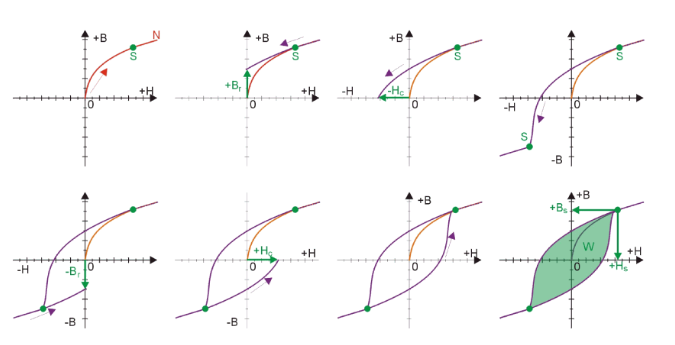
\includegraphics[scale=0.3]{./figures/hysterese.png}
	\caption{Hysteresekurve eines Ferromagneten ([1] p.10 Abb. 6)}
	\label{fig:hysterese}
\end{figure}

\noindent
Die Magnetisierung kann durch 4 in Abbildung \ref{fig:hysterese} zu sehenden Werte charakterisiert werden.\\
$B_r$ \ldots der Ordinatenabschnitt\\
$H_c$ \ldots der Abszissenabschnitt\\
$B_S, H_S$ \ldots die Koordinaten des Sättigungspunktes\\

% TODO mu_0, mu_r, Formel dafür umformen PAT

\textbf{Berechnung Suszeptilität von Graphit nach Fraraday}

$$\chi_{Faraday} = \frac{F \cdot \mu_0}{V \cdot B \cdot \frac{dB}{dx}}$$
$\mu_0$ \ldots magnetische Konstante\\
$F$ \ldots Kraft auf Probe\\
$V$ \ldots Probevolumen\\
$B$ \ldots Magnetische Flussdichte\\

\noindent \textbf{Berechnung Suzeptibilität von Graphit nach Gouy}

$$\chi = \frac{A \cdot B^2(x_2)}{F_x \cdot 2 \cdot \mu_{0}} $$
Da der Messaufbau eine Rechnung mit dieser Variante nicht zugelassen hat, wird hier nicht näher darauf eingegangen und auf die Herleitung ([1] p.12 Formeln 9-11) verwiesen.\\

\noindent \textbf{Darstellen der Hystereseschleife:}\\
Eine Wechselspannung wird an einen Transformator mit Eisenkern angelegt. Die Spannungen an der Primär und an der Sekundärspule werden am Oszilloskop dargestellt.\\
Durch die Funktionsweise eines Transformators ergibt sich im ferromagnetischen Trafo-Kern die Hystereseschleife:\\
Die Primärspule erzeugt ein äußeres Magnetfeld H. Dieses magnetisiert den Kern. Das B-Feld des Kerns induziert wiederum eine Spannung in der Sekundärspule.\\
Da diese Induktionsvorgänge von verschiedenen Faktoren, wie Windungszahlen, Spulenlänge, Spulenwiderstand, oder auch Querschnittsfläche und Volumen des Kerns die Spannungen und Magnetfelder in linearen Zusammenhang bringen, lässt sich die Magnetisierung des Kerns direkt aus den Spannungen darstellen (eben mit linearen Umrechnungsfaktoren):
$$H(t) = \frac{n_1}{L R_v}\cdot U_{primaer}(t)$$
$$B(t)= \frac{R\cdot C}{n_2 \cdot A} \cdot U_{sekundaer}(t)$$
Alle Parameter sind in [1] zu finden, die Funktionsweise und Anwendungen des Transformators werden in PW10 erklärt.
\pagebreak
%%%%%%%%%%%%%%%%%%%%%%%%%%%%%%%%%%%%%%%%%%%%%%%%%%%%%%%%%%%%%%%%%%%%%%%
\subsection{Resultate}
\textbf{Messung der Suszeptilität von Graphit:}\\
(vom Betreuer angegebene Werte, wegen eines Defekts der Magnetfeldsonde:)\\
$B = (0.6 \pm 0.1)T$\\
$\frac{dB}{dx} = (40 \pm 1) \frac{T}{m}$\\
\\
% TODO Fehler (Shorty diesmal PLZ, übung ftw :)
\textbf{Polykristalines Graphit:}\\
$V=(0.35 \pm 0.05) ml$\\
$F_x=(-0.50 \pm 0.06)mN$

$$\chi_{poly} = (-7.482 \cdot 10^{-5} \pm 1.4 \cdot 10^{-5})$$

\textbf{Pyrolythisches Graphit:}\\
$V=(0.20 \pm 0.01) ml$\\
$F_x=(-1.24 \pm 0.06)mN$
$$\chi_{pyro} = (-3.247 \cdot 10^{-4} \pm 1.363 \cdot 10^{-4})$$
\\
\noindent
\textbf{Trafo W}\\

\end{multicols}
\begin{figure}[H]
	\centering
	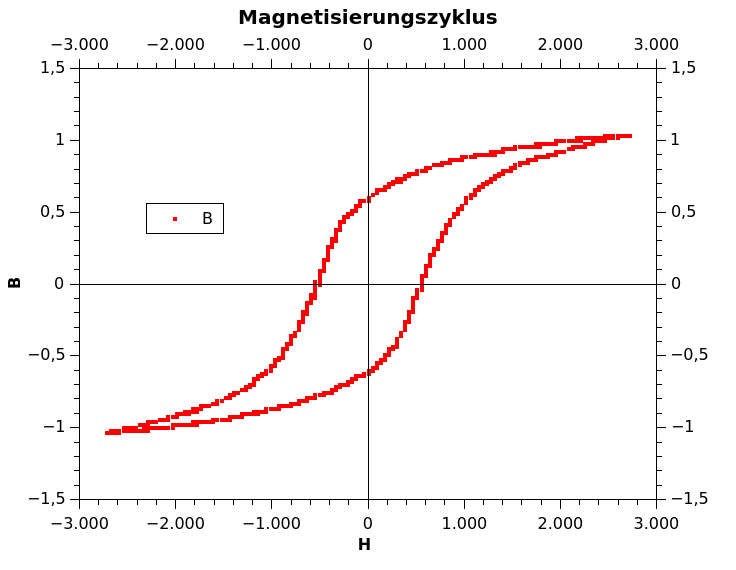
\includegraphics[scale=1]{./figures/Trafo_W_Hysterese.png}
	\caption{Hysteresekurve des Ferromagneten W}
	\label{fig:Trafo_W_Hysterese}
\end{figure}
\begin{figure}[H]
	\centering
	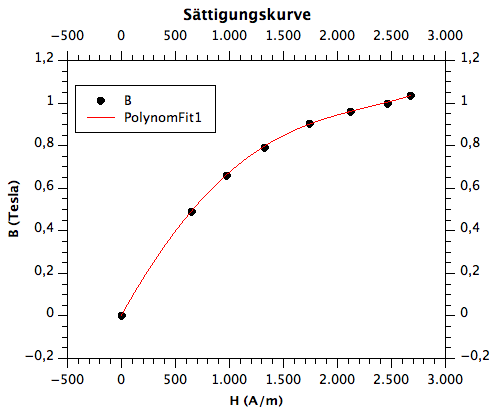
\includegraphics[scale=0.7]{./figures/Trafo_W_saettigung02.png}
	\caption{Sättigungskurve mit künstlichem Nullpunkt zur Bestimmung von $\mu_r$}
	\label{fig:Trafo_W_saettigung}
\end{figure}
\begin{figure}[H]
	\centering
	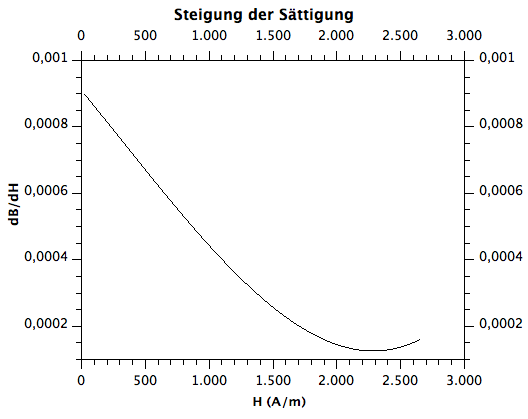
\includegraphics[scale=0.6]{./figures/Trafo_W_saettigung-steigung.png}
	\caption{Sättigungskurve mit künstlichem Nullpunkt zur Bestimmung von $\mu_r$}
	\label{fig:Trafo_W_saettigung}
\end{figure}
\begin{multicols}{2}
%TODO Fehler = skalierung im Graphen
$$B_r = (0.577 \pm 0.00471)T$$
$$H_c = (554.35 \pm 1.05)\frac{V}{m}$$
$$B_S = (1.0358 \pm 0.00471)T$$
$$H_S = (2728.26 \pm 1.05)\frac{V}{m}$$

%TODO da war noch was mit integrieren der Kurve?!

\noindent
Die Rohdaten und QTI-Auswertungen sind unter [2] zu finden.

%%%%%%%%%%%%%%%%%%%%%%%%%%%%%%%%%%%%%%%%%%%%%%%%%%%%%%%%%%%%%%%%%%%%%%%
\subsection{Diskussion}
\textbf{Suszeptibilität:}\\
Durch eine defekte B-Feld Sonde konnte die Messung nach Gouy leider nicht durchgeführt werden. Das Ergebnis für das Diamagnetika Graphit war mit der Methode nach Faraday gerade noch im Messbereich der Geräte feststellbar. Trotz Anmerkung in [1] war die geringe Krafteinwirkung überraschend. Ein Unterschied bei polykristalinen und pyrolythischem Graphit ging in den Ergebnissen hervor.\\

Die Abschätzung der Messunsicherheit der Kraftwirkung beruht auf den Fluktuationen der Kraft auf die Probe. Die Auflösung des Sensors selbst wäre deutlich geringer ($\pm 0.01mN$, abgeschätzt wurde auf (\pm 0.06mN$)
\\
Ein weiterer Faktor ist der große resultierende Fehler bei den gegebenen Werten, da diese wie der z.B. der Gradient aus einem Plot geschätzt wurde ($\pm 1\frac{t}{m}$).

\textbf{Sättigungskurve}\\
Die Bestimmung der Sättigungspunkte für verschiedene Spannungen und Ströme wurde durch das Oszilloskop erleichtert. Ein fehlverhalten im Drehregler des Netzgerätes sorgte leider für einen Sprung von 0mA auf 43mA was eine genaue Bestimmung der Steigung am Nullpunkt nicht möglich machte. Durch einfügen eines Punktes in (0,0) konnte jedoch ein Polynomfit 4-ter Ordnung durchgeführt werden. % TODO mu_0 zu literaturwert


\section{Quellen}
$[1]$ Anleitung, \url{http://www.univie.ac.at/anfpra/neu1/ps/ps12/PS12.pdf}\\
$[2]$ Rohdaten, \url{htts://github.com/blackandcold/Protocols-SS2014-P2/tree/master/PS_12/data}\\

\end{multicols}
\end{document}